\section{Проект}
\subsection{Средства реализации}
Для реализации приложения был выбран язык программирования C++, т.к. он очень распространен, что упрощает последующую поддержку приложения. К тому же, программы, написанные на этом языке, могут быть скомпилированы для очень большого количества платформ.

Для упрощения переноса приложения на другие платформы, был использован кроссплатформенный инструментарий разработки ПО под названием Qt. Он так же включает в себя инструментарий, необходимый для разработки кроссплатформенных приложений с графическим интерфейсом пользователя. Выбор этого инструментария позволяет уменьшить усилия, требуемые для реализации новой и поддержки имеющейся функциональности.

Для того, чтобы приложение могло задействовать как можно больше доступных ресурсов современных ПК, было решено использовать фреймворк OpenCL. Это позволит приложению задействовать ресурсы всех процессоров в многопроцессорных системах, а так же ресурсы современных видеокарт.
Для взаимодействия с OpenCL используется библиотека OpenCLxx~\cite{opencl_openclxx}, которая предоставляет ООП-интерфейс для доступа к OpenCL.

\subsection{Модули и алгоритмы}

\subsubsection{Классы приложения}
\begin{itemize}
\item \textit{MainWindow} -- главное окно приложения
\item \textit{ImageInfo} -- информация об изображении
\item \textit{ImagePreview} -- виджет предпросмотра изображений
\item \textit{ImageScene} -- сцена для отображения изображения
\end{itemize}

\subsubsection{Класс MainWindow}
Методы класса:
\begin{itemize}
\item \textit{add\_image} -- добавление нового изображения
\item \textit{load\_metafile} -- загрузка метафайла
\item \textit{save\_metafile} -- сохранение метафайла
\end{itemize}

\subsubsection{Класс ImagePreview}
Методы класса:
\begin{itemize}
\item \textit{add\_image} -- добавление нового изображения в блок предпросмотра
\item \textit{clear} -- очистка блока предпросмотра
\end{itemize}

\subsubsection{Класс ImageScene}
Методы класса:
\begin{itemize}
\item \textit{rectangle\_changed} -- изменяет параметры объемлющего прямоугольника для изображения
\item \textit{set\_rectangle} -- устанавливает объемлющий прямоугольник для отображения
\item \textit{set\_image} -- устанавливает изображение для отображения
\end{itemize}

\subsection{Проект интерфейса}
Из меню графического интерфейса пользователя должно быть доступно сохранение и загрузка метафайла, добавление нового изображения, запуск на выполнение алгоритма получения объемной модели объекта. Основное окно должно быть разделено на три части: слева должны находиться блок предпросмотра изображений и блок ввода матрицы внешней калибровки камеры для выбранного изображения. Остальную часть окна должен занимать блок, в который выводится текущее выбранное изображение. Так же в этом блоке должно быть доступно выделение объемлющего прямоугольника.
\renewcommand{\figurename}{Рис.}
\begin{figure}[h]
\center
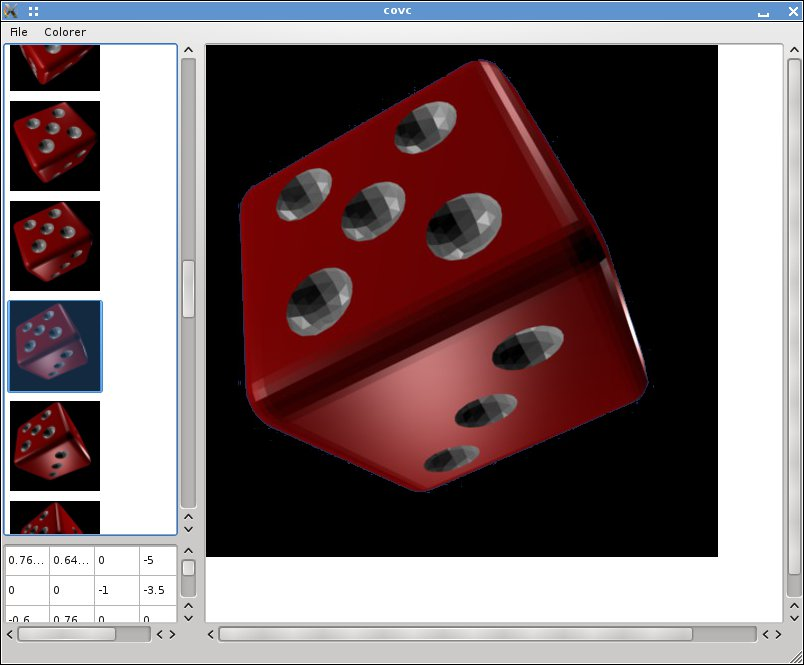
\includegraphics[scale=0.5]{gui}
\caption{Проект интерфейса}
\end{figure}

